

%%%%%%%%%%%%%%%%%%%%%%%%%%%%%%%%%%%55%%
\begin{frame} [plain]
    \frametitle{}
    \Background[1] 
    \begin{center}
    {\huge 第3讲:量子力学基础}
    \end{center}  
    \addtocounter{framenumber}{-1}   
\end{frame}
%%%%%%%%%%%%%%%%%%%%%%%%%%%%%%%%%%

\section{1.量子态与希尔伯特空间}

\begin{frame} 
    \frametitle{希尔伯特空间}
    量子态用希尔伯特空间中矢量描述\\
    \begin{equation*}
        \begin{split}
            \text{1、定义加法} \quad  &\xi=\psi+\varphi\\
            &\psi+\varphi=\varphi+\psi \qquad (\text{交换律})\\
            &(\psi+\varphi)+\xi=\psi+(\varphi+\xi) \qquad (\text{结合律})\\
            &\psi+\text{O}= \psi \qquad (\text{零元})\\
            &\psi+\varphi= \text{O} \qquad (\text{逆元})\\
        \end{split}  
    \end{equation*}
\end{frame} 

\begin{frame} 
    \begin{equation*}
        \begin{split}
            \text{2、定义数乘} \quad &\varphi=\psi a\\
            &\psi 1= \psi \qquad (\text{1元})\\
            &(\psi a)b=\psi (ab) \qquad (\text{结合律})\\
            &\psi(a+b)= \psi a+ \psi b \qquad (\text{第一分配律})\\
            &(\psi+\varphi) a= \psi a +\varphi a \qquad (\text{第二分配律})\\
        \end{split}  
    \end{equation*}
\end{frame} 

\begin{frame} 
    \begin{equation*}
        \begin{split}
            \text{3、定义内积} \quad &c=(\psi, \varphi)\\
            &(\psi, \varphi)= (\varphi,\psi)^* \\
            &(\psi, \varphi+\xi)= (\psi, \varphi) + (\psi, \xi)\qquad (\text{分配律})\\
            &(\psi, \varphi a)= (\psi, \varphi )a \\
            &\Rightarrow (\psi a, \varphi )= (\psi, \varphi )a^* \\
            &(\psi,\psi)= c\ge 0\\
        \end{split}  
    \end{equation*}
\end{frame}

\begin{frame} 
    \例 [1. 有定义在$C^n$空间的列矩阵,求内积]
    { \[\psi=
        \begin{pmatrix}
                a_1\\
                a_2\\
                a_3
        \end{pmatrix}, \qquad 
        \varphi =\begin{pmatrix}
            b_1\\
            b_2\\
            b_3
    \end{pmatrix}
     \] 
    }
    \解 ~ \[(\psi, \varphi) = \begin{pmatrix}
        a_1 ^* &
        a_2 ^* &
        a_3 ^*
    \end{pmatrix}
        \begin{pmatrix}
        b_1\\
        b_2\\
        b_3
    \end{pmatrix}
    =a_1 ^* b_1 +a_2 ^* b_2 +a_3 ^* b_3
    =c 
    \]
    ~ \[(\varphi,\psi) = \begin{pmatrix}
        b_1 ^* &
        b_2 ^* &
        b_3 ^*
    \end{pmatrix}
        \begin{pmatrix}
        a_1\\
        a_2\\
        a_3
    \end{pmatrix}
    =b_1 ^* a_1 +b_2 ^* a_2 +b_3 ^* a_3
    =c^* 
    \]
\end{frame} 

\begin{frame} 
    \例 [2. 求定义在x空间的函数的内积]{}

    \解 ~ \[(\psi, \varphi)=\int_a ^b \psi^*(x)  \varphi(x) dx
    =c 
    \]
    ~ \[(\psi, \varphi)=\int_a ^b \varphi^*(x)\psi(x) dx = (\int_a ^b \varphi(x)\psi^*(x) dx) ^* =c^*\]
\end{frame} 

\begin{frame}
    4、定义空间\\
   \begin{itemize}
       \Item 矢量空间:满足加法和数乘两种运算的集合
       \Item 内积空间:满足加法、数乘和内积三种运算的集合
       \Item 希尔伯特空间:  完全的内积空间\\
       ~~ \\
       *完全性:对给定任意小的实数$\varepsilon$,总有数N存在,当m, n>N时,有\\
       $$ (\psi_m -\psi_n, \psi_m -\psi_n )< \varepsilon $$
   \end{itemize} 
   \Tips ~ 量子体系的状态用希尔伯特空间的矢量描述
\end{frame} 

\begin{frame}
    5、几个概念\\
   \begin{itemize}
       \Item 模(方):$|\psi|^2= (\psi, \psi)=c$
       \Item 归一化: $|\psi|^2= (\psi, \psi)=c=1$
       \Item 正交(线性无关)性:  $(\psi, \varphi)=0 $ \\
       \Item 完全集: 有一组线性无关集,如果空间的任意矢量都可以在其上展开,则称它为一个完全集,记为$\{\phi_i\}$ 
       \[\psi=\sum_i a_i \phi_i= \sum_i (\phi_i,\psi) \phi_i\]
       \Item 维度:最小完全集所包含矢量的数目相同,称这个数目为空间的维度
       \Item 正交归一完全集:对于一个n维的完全集,有:\[(\phi_i,\phi_j)=\delta_{ij}, \qquad i,j=1,2,3,\cdots, n \]
       \Item 基与基矢:称一个正交归一完全集为空间的一个基,它所含的矢量称不计算基矢(态)
   \end{itemize} 
\end{frame} 

\begin{frame}
 \Tips~ 同一空间可以有不同的基,\\
 $C^2$空间的一个基:
 \[ \rs{0}\equiv\begin{bmatrix}
     1 \\
     0
 \end{bmatrix}; \qquad \rs{1}\equiv\begin{bmatrix}
    0 \\
    1
\end{bmatrix} \]

$C^2$空间的另一个基:
\[ \rs{+}\equiv\frac{1}{\sqrt{2}}\begin{bmatrix}
    1 \\
    1
\end{bmatrix}=\Pstate; \qquad \rs{-}\equiv\frac{1}{\sqrt{2}}\begin{bmatrix}
   1 \\
   -1
\end{bmatrix}=\Mstate \]

\end{frame} 

\begin{frame} 
    \begin{center}
        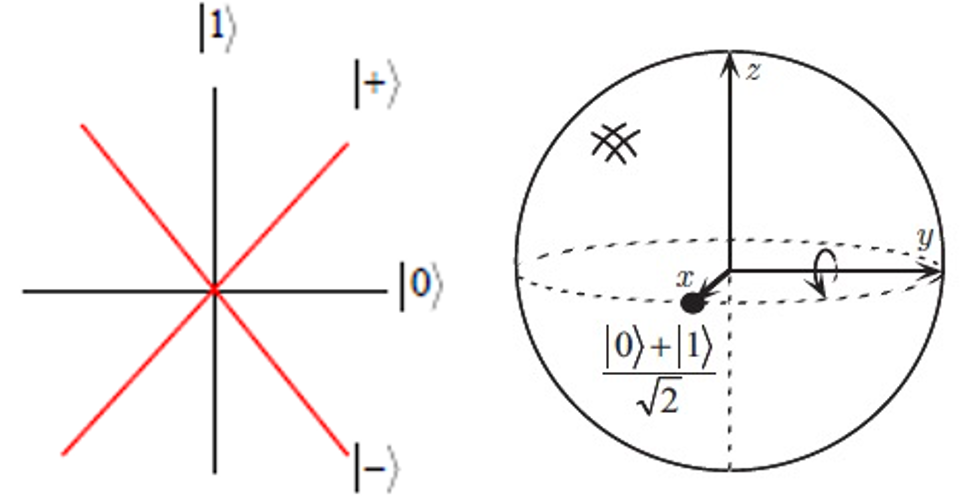
\includegraphics[width=0.7\textwidth]{figs/26.png}
    \end{center} 
\end{frame}


\begin{frame}{}
    6、左矢与右矢\\
    考察内积: $(\psi,\psi)=\int\psi^*\psi d\tau$ \\
    同一波函数放在左边还是右边,意义有所不同: \\
    右边是线性的:  $(\psi,a\psi)=a (\psi,\psi)$ \\
    左边是反线性的:   $(a\psi,\psi)=a^* (\psi,\psi)$  \\
    为了清楚地描述这种线性反线性特点,定义左矢和右矢
    $$\langle \psi |, \qquad |\psi \rangle $$ 
    内积:\[(\psi,\varphi)\equiv \langle \psi | \varphi \rangle\]
    有性质: $$\langle a\psi | = \langle \psi |a^* $$
    $$ |a\psi \rangle = a|\psi \rangle$$ 
\end{frame}

\begin{frame}{}
    7、外积\\
    考察展开式: \[\psi=\sum_i a_i \phi_i= \sum_i (\phi_i,\psi) \phi_i\]
    \[\rs{\psi}=\sum_i a_i \rs{\phi_i}= \sum_i \lr{\phi_i}{\psi} \rs{\phi_i} =\sum_i \rl{\phi_i}{\phi_i} \rs{\psi}\]
    ~~\\
    令 $p_i= \rl{\phi_i}{\phi_i} $, 完备性:
    \[\sum_i p_i= \sum_i \rl{\phi_i}{\phi_i}=1 \]
    称  $p_i= \rl{\phi_i}{\phi_i} $ 外积
\end{frame}

\begin{frame}{}
        \例 [3. 有定义在$C^n$空间的列矩阵,求内积和外积]
        { \[\rs{\psi}=
            \begin{pmatrix}
                    a_1\\
                    a_2\\
                    a_3
            \end{pmatrix}, \qquad 
            \rs{\varphi} =\begin{pmatrix}
                b_1\\
                b_2\\
                b_3
        \end{pmatrix}
         \] 
        }
        \解 ~ \[\lr{\psi}{\varphi} = \begin{pmatrix}
            a_1 ^* &
            a_2 ^* &
            a_3 ^*
        \end{pmatrix}
            \begin{pmatrix}
            b_1\\
            b_2\\
            b_3
        \end{pmatrix}
        =a_1 ^* b_1 +a_2 ^* b_2 +a_3 ^* b_3
        =c 
        \]
        ~ \[\rl{\psi}{\varphi} = \begin{pmatrix}
            a_1  \\
            a_2  \\
            a_3 
        \end{pmatrix}
            \begin{pmatrix}
            b_1 ^* &
            b_2 ^* &
            b_3 ^*
        \end{pmatrix}
        =  \begin{pmatrix}
            a_1b_1 ^* & a_1b_2 ^* & a_1b_3 ^* \\
            a_2b_1 ^* & a_2b_2 ^* & a_2b_3 ^* \\
            a_3b_1 ^* & a_3b_2 ^* & a_3b_3 ^* 
        \end{pmatrix}
        \]
    \Tips ~ 内积是一个数,外积是一个矩阵!
\end{frame}

\section{2.物理量与算符}

\begin{frame}
    \frametitle{算符}
    物理量用希尔伯特空间的线性厄密算符描述\\
    1. 定义:
    \begin{itemize}
        \Item 算符:描述态矢量之间的映射关系,即算符作用于一个态矢量,映射到另一个态矢量。
        \[F \rs{\Psi}=\rs{\psi}\]
        \Item 逆算符  
        \[F^{-1}\rs{\psi}=\rs{\Psi} \] 
        \Item 线性算符 \[F (a\rs{\Psi} +b\rs{\psi}) = aF \rs{\Psi} +bF\rs{\psi}\]
        \Item 伴算符   \[\ls{\psi}=\ls{\Psi}F^{\dagger} \]
    \end{itemize}
\end{frame} 


\begin{frame}
    \frametitle{}
    \begin{itemize}
        \Item 自伴(厄密)算符  \[F = F^{\dagger} \] 性质: $\lr{\Psi F}{\psi}=\lr{\Psi }{F \psi}=\lcr{\Psi }{F} {\psi}$
        \Item 幺正(酉)算符    \[F^{-1} = F^{\dagger} \] 性质: $FF^{\dagger}=F^{\dagger}F=I$, 通常写成 $UU^{\dagger}=U^{\dagger}U=I$ \\ \vspace{1.0em}
    \end{itemize}        
    \Tips 把一个空间所有矢量都用同一幺正算符作用,得到一个新的空间, 即幺正(酉)变换是一种空间变换,
        \[U\rs{\Psi} =\rs{\Psi'}\]
\end{frame} 
\begin{frame}
    \frametitle{}
    {\Bullet}~新旧空间算符之间的关系: \\
        旧空间的算符: \[F \rs{\Psi}=\rs{\varphi}\]
        新空间的算符: \[F' \rs{\Psi'}=\rs{\varphi'}\]
        它们之间的关系:
        \[F' U\rs{\Psi}=U\rs{\varphi}\]
        \[F' U\rs{\Psi}=UF \rs{\Psi}\]
        \[U^{\dagger}F' U\rs{\Psi}=U^{\dagger}UF \rs{\Psi}\]
        \[U^{\dagger}F' U\rs{\Psi}=IF \rs{\Psi}\]
        \[U^{\dagger}F' U=F \]
        %\item 
\end{frame}

\begin{frame}
    \frametitle{}
    \begin{itemize}
    \Item 投影算符: 基矢的外积是一种投影算符,
    \end{itemize}
    对于展开式: 
    \[\rs{\psi}=\sum_i a_i \rs{\phi_i}=\sum_i \rl{\phi_i}{\phi_i} \rs{\psi}=\sum_i p_i \rs{\psi} =\sum_i \rs{\psi_i}\]
    有:\[p_i \rs{\psi} =\sum_i \rs{\psi_i}\]
    即,外积$\rl{\phi_i}{\phi_i}$作用于$\rs{\psi}$,得到其在第$i$个基矢态上的投影分量!\\
\end{frame}

\begin{frame}    
    \begin{itemize}
        \Item 测量算子: 量子信息学中常称投影算符为测量算子,定义为
        \end{itemize}
    \[M_0=\rl{0}{0}, \qquad M_1=\rl{1}{1} \]
    具有$2\times 2$的矩阵形式,
    可以证明:\\
    {\bullet} 测量算子是自伴(厄密)算符 :\[M_m = M_m ^{\dagger} \]
    {\bullet} 平方不变性 :\[M_m ^2 = M_m \]
    {\bullet} 完备性 :\[M_0 + M_1 = M_0 ^2 + M_1 ^2 = M_0 M_0 ^\dagger + M_1 M_0 ^\dagger=I\]
\end{frame}

\begin{frame} 
    \frametitle{}
    {\bullet} 测量后的态函数 
    \[\begin{aligned}
        M_0\rs{\Psi} 
        &= \rl{0}{0}(a_0\rs{0}+a_1\rs{1})  \\ 
        &= \rl{0}{0}a_0\rs{0}  \\ 
        &= a_0\rs{0}  \\ 
        &= \frac{a_0}{|a_0|}\rs{0}  \qquad \text{(归一化)} \\ 
    \end{aligned}\]    
    {\bullet} 测得的概率(密度) 
    \[\begin{aligned}
        \lcr{\Psi}{M_0 ^\dagger M_0}{\Psi} 
        &= \lcr{0 }{a_0a_0} {0} \\ 
        &= \lr{0 }{0}a_0 ^* a_0 \\ 
        &= |a_0|^2 = p(0) 
    \end{aligned}\] 
    重写测量后的状态 \[  M_m\rs{\Psi} = \frac{a_m\rs{m}}{\sqrt{\lcr{\Psi}{M_m ^\dagger M_m}{\Psi}}} = \frac{M_m\rs{\Psi}}{\sqrt{\lcr{\Psi}{M_m ^\dagger M_m}{\Psi}}}\]
\end{frame}

\begin{frame}
    \frametitle{}
    \begin{itemize}
    \Item 密度算符: 任意态的外积是一种求概率密度的算符,简称密度算符,
    \end{itemize}
    任意态的展开式:\[\rs{\psi}=\sum_i a_i \rs{\phi_i}\]
    任意态的外积:\[\rho=\rl{\psi}{\psi}\]
    求其在基矢态上的平均值:
    \[\lcr{\phi_i}{\rho}{\phi_i}=\lcr{\phi_i}{\rl{\psi}{\psi}}{\phi_i}=\lr{\phi_i}{\psi}\lr{\psi}{\phi_i}
    =a_i ^* a_i =|a_i|^2=\omega_i     
    \]    
    密度算符的应用,平均值公式-3 
    \[\overline{F}=tr(A\rho)\]
\end{frame}


\begin{frame}
    \frametitle{}
    2. 算符的矩阵表示
    \[\begin{aligned}
        \rs{\psi}&=F \rs{\Psi} \\
        \lr{i}{\psi}&= \lcr{i}{F}{\Psi} \\
        \lr{i}{\psi}&= \sum_j\lcr{i}{F}{j}\lr{j}{\Psi} \\
        \rs{\psi_i}&= \sum_j F_{ij}\rs{\Psi_j} 
    \end{aligned}\]  
    定义了算符矩阵元公式:\[ F_{ij}=\lcr{i}{F}{j}\]
    伴算符的矩阵等于原算符的厄密共轭:\[ F^{\dagger}=(F_{ij} ^*)^T\]
\end{frame}


\begin{frame}
    \frametitle{}
    \例[4.证明平均值公式-3 ]{
    \[\overline{F}=tr(A\rho)\]}
    \证~由矩阵的迹的定义式  
    \[\begin{aligned}
        tr(A\rho) &= \sum_i \lcr{i}{A\rho}{i} \\
        &= \sum_i \lcr{i}{A}{\psi}\lr{\psi}{i} \\
        &= \sum_i \lr{\psi}{i} \lcr{i}{A}{\psi}\\
        &= \lcr{\psi}{A}{\psi}\\
    \end{aligned}\]    
\end{frame}

\begin{frame}
    \frametitle{}
    3. 算符的本征方程
    \begin{itemize}
        \Item 定义式: \[F \rs{\Psi}=f\rs{\Psi}\]
        \Item 相关定理:
        \begin{itemize}
            \IItem 厄密算符的本征值是实数
            \IItem 厄密算符的所有本征矢构成正交归一完全集
            \IItem 当且仅当两厄密算符互相对易时才且有共同的
            本征矢完全集
            \IItem 完全确定一个量子态所需要的彼此对易的一组力学量算符的最小集称为力学量完全集,所含力学量数目与体系的自由度数目相同
            \end{itemize}
    \end{itemize}
\end{frame}

\section{3.张量空间}

\begin{frame}
    \frametitle{张量空间}
    **以上讲的是单粒子体系的量子态及物理量的描述问题
    \begin{tcolorbox4}[张量积]
    对于多粒子体系,比如多量子比特系统,其所处的空间是子系统希尔伯特空间的张量积。也称直积空间。
    \end{tcolorbox4}
\end{frame}

\begin{frame}
    \frametitle{}
    1. 张量空间的计算基矢 \\
    子系统A是n维的,计算基(某厄密算符的本征函数系)为$$\{\rs{\phi_i}\},\quad (i=1,2,3,\cdots,n)$$ 
    子系统B是m维的,计算基为$$\{\rs{\varphi_j}\},\quad (j=1,2,3,\cdots,m)$$ 
    总系统是n张m维的张量空间,计算基为:$$\{\rs{\phi_i}\otimes\rs{\varphi_j}\},\quad (i=1,2,3,\cdots,n;\quad j=1,2,3,\cdots,m)$$ 
    可简写为:$$\{\rs{\phi_i}\otimes\rs{\varphi_j}\}=\{\rs{\phi_i}\rs{\varphi_j}\}=\{\rs{\phi_i\varphi_j}\}=\{\rs{ij}\}$$
\end{frame}

\begin{frame}
    \frametitle{}
    总体系的任意态是计算基矢的叠加态:
    \[ \rs{\Psi} = \sum_{i,j} ^{n,m} a_{ij}\rs{ij}\] \vspace{0.6em}

    \例[写出双量子比特的计算基]{} 
    \解~双量子比特的基由四个计算基矢构成$$\{\rs{00},\rs{01},\rs{10},\rs{11}\}$$
    它们的矩阵形式为:
    \[
\rs{00} = 
\begin{pmatrix}
    1\\
    0\\
    0\\
    0
\end{pmatrix},\qquad
\rs{01} = 
\begin{pmatrix}
    0\\
    1\\
    0\\
    0
\end{pmatrix},\qquad
\rs{10} = 
\begin{pmatrix}
    0\\
    0\\
    1\\
    0
\end{pmatrix},\qquad
\rs{1} = 
\begin{pmatrix}
    0\\
    0\\
    0\\
    1
\end{pmatrix}
\] 
\end{frame}

\begin{frame}
    \frametitle{}
    双量子比特是四个计算基矢的叠加态:
    \[\rs{\psi} =\alpha_{00}\rs{00}+\alpha_{01}\rs{01}+\alpha_{10}\rs{10}+\alpha_{11}\rs{11}\]
    归一化条件:
    \[ \sum_{ij=0,1} |\alpha_{ij}|^2= 1\]
    ~~\\
    2. 张量空间的算符 \\
    子系统A有算符$F_A$, 子系统B有算符$F_B$,总系统可定义它们的张量积
    \[F_{AB}=F_A \otimes F_B\]
    作用于总体系的任意态时,算法为:
    \[F_A \otimes F_B \rs{\Psi} = F_A \otimes F_B \sum_{i,j} a_{ij}\rs{ij}=  \sum_{i,j} a_{ij}F_A \rs{i}\otimes F_B\rs{j}\]   
\end{frame}

\begin{frame}
    \frametitle{}
    3. 子系统的测量与约化密度矩阵 \\
    总体系任意态的密度矩阵
    \[ \rho=\rl{\Psi} {\Psi}= \sum_{i,i',j,j'} a_{i'j'}a_{ij}\rl{i'j'}{ij}\] 
    定义子体系A的约化密度矩阵(把子系统B积分丢!)
    \[ \rho(A)=\sum_{j}\lcr{j}{\rho}{j}=tr_B(\rho)\] 
    测量子体系A的物理量$F_A$的平均值为:
    \[ \bar{F}_A=tr_A(F_A\rho(A))\] 
    
\end{frame}



\section{4.量子力学基本假设}

\begin{frame}
    \frametitle{状态假设}
    \begin{tcolorbox4}[1. 状态假设]
    量子体系的状态用希尔伯特空间的态矢量完全描述。
    \end{tcolorbox4}
    \例[量子比特用2维希尔伯特空间的态矢量]{ 
    \[\rs{\psi} = a_0 \rs{0} + a_1\rs{1}\]完全描述了体系所有可能的状态!}
\end{frame}


\begin{frame}
    \frametitle{演化假设}
    \begin{tcolorbox4}[2. 演化假设]
    一个封闭量子体系的演化用幺正(酉)变换描述。
    \[\rs{\Psi'}=U\rs{\Psi}\]
    状态函数随时间的演化用薛定谔方程描述
    \[ i\hbar \frac{d\rs{\Psi}}{dt}=H \rs{\Psi}\]
    \end{tcolorbox4}
\end{frame}

\begin{frame}
    \例[试证明薛定谔方程与酉变换等价]{}
    \证~ 定义时间演化算符:
    $$ U(t,t_0) |\Psi(t_0)\rangle = |\Psi(t)\rangle  $$
    \alert{分析}:
    (1) 因为 $ U(t_0,t_0) |\Psi(t_0)\rangle = |\Psi(t_0)\rangle  $ \\
    $$ U(t_0,t_0)=I $$
    (2):求 $ U(t,t_0)$
    $$ \begin{aligned}
        i\hbar \frac{\partial }{\partial t} |\Psi(t)\rangle &= H|\Psi(t)\rangle  \\
        i\hbar \frac{\partial }{\partial t}  U(t,t_0) |\Psi(t)\rangle &= H U(t,t_0) |\Psi(t)\rangle  \\
        i\hbar \frac{\partial }{\partial t}  U(t,t_0)  &= H U(t,t_0)  \\
        U(t,t_0)  &= e^{-\frac{i}{\hbar} H(t-t_0)}  \\
    \end{aligned} $$
\end{frame}

\begin{frame}  
    (3):$ U(t,t_0)$是幺正算符
    $$ \begin{aligned}
        U(t,t_0)  &= e^{-\frac{i}{\hbar} H(t-t_0)}  \\
        U^\dagger (t,t_0)  &= e^{\frac{i}{\hbar} H(t-t_0)}  \\
        U^\dagger (t,t_0)U(t,t_0) &= U^\dagger (t,t_0)U(t,t_0) \\
         &=e^{\frac{i}{\hbar} H(t-t_0)-\frac{i}{\hbar} H(t-t_0)} \\
         &=e^0 \\
         &=I
    \end{aligned} $$
    因此,有:
    $$ |\Psi(t)\rangle = U(t,t_0) |\Psi(t_0)\rangle   $$
    \Note ~波函数随时间的演化服从的薛定谔方程,只是一种幺正变换。
\end{frame} 

\begin{frame}
    \frametitle{量子测量假设}
    \begin{tcolorbox4}[3. 量子测量假设]
    量子测量由一组测量算子$\{ M_m\}$ 描述,测得测量值$m$的概率(密度)为
    \[ p(m)=\lcr{\Psi}{M_m ^\dagger M_m}{\Psi} 
     \]
     测量后的状态 \[\frac{M_m\rs{\Psi}}{\sqrt{\lcr{\Psi}{M_m ^\dagger M_m}{\Psi}}}\]
    \end{tcolorbox4}
\end{frame}

\begin{frame}
    \frametitle{张量积假设}
    \begin{tcolorbox4}[4. 复合系统假设]
    复合系统的状态空间是子系统的状态空间的张量积
    \end{tcolorbox4}
\end{frame}

\begin{frame}
    \frametitle{}
    \begin{tcolorbox3}[学术讨论]
        基于以上4个假定,可以从数学上在Hilbert空间导出整个量子力学体系,那么基于假定导出的量子力学可靠吗?
    \end{tcolorbox3}
\end{frame}